\documentclass[11,]{article}
\usepackage{lmodern}
\usepackage{amssymb,amsmath}
\usepackage{ifxetex,ifluatex}
\usepackage{fixltx2e} % provides \textsubscript
\ifnum 0\ifxetex 1\fi\ifluatex 1\fi=0 % if pdftex
  \usepackage[T1]{fontenc}
  \usepackage[utf8]{inputenc}
\else % if luatex or xelatex
  \ifxetex
    \usepackage{mathspec}
    \usepackage{xltxtra,xunicode}
  \else
    \usepackage{fontspec}
  \fi
  \defaultfontfeatures{Mapping=tex-text,Scale=MatchLowercase}
  \newcommand{\euro}{€}
\fi
% use upquote if available, for straight quotes in verbatim environments
\IfFileExists{upquote.sty}{\usepackage{upquote}}{}
% use microtype if available
\IfFileExists{microtype.sty}{%
\usepackage{microtype}
\UseMicrotypeSet[protrusion]{basicmath} % disable protrusion for tt fonts
}{}
\usepackage[margin=1.0in]{geometry}
\usepackage{graphicx}
\makeatletter
\def\maxwidth{\ifdim\Gin@nat@width>\linewidth\linewidth\else\Gin@nat@width\fi}
\def\maxheight{\ifdim\Gin@nat@height>\textheight\textheight\else\Gin@nat@height\fi}
\makeatother
% Scale images if necessary, so that they will not overflow the page
% margins by default, and it is still possible to overwrite the defaults
% using explicit options in \includegraphics[width, height, ...]{}
\setkeys{Gin}{width=\maxwidth,height=\maxheight,keepaspectratio}
\ifxetex
  \usepackage[setpagesize=false, % page size defined by xetex
              unicode=false, % unicode breaks when used with xetex
              xetex]{hyperref}
\else
  \usepackage[unicode=true]{hyperref}
\fi
\hypersetup{breaklinks=true,
            bookmarks=true,
            pdfauthor={},
            pdftitle={NAME OF THIS STUDY},
            colorlinks=true,
            citecolor=blue,
            urlcolor=blue,
            linkcolor=magenta,
            pdfborder={0 0 0}}
\urlstyle{same}  % don't use monospace font for urls
\setlength{\parindent}{0pt}
\setlength{\parskip}{6pt plus 2pt minus 1pt}
\setlength{\emergencystretch}{3em}  % prevent overfull lines
\setcounter{secnumdepth}{0}

%%% Use protect on footnotes to avoid problems with footnotes in titles
\let\rmarkdownfootnote\footnote%
\def\footnote{\protect\rmarkdownfootnote}

%%% Change title format to be more compact
\usepackage{titling}

% Create subtitle command for use in maketitle
\newcommand{\subtitle}[1]{
  \posttitle{
    \begin{center}\large#1\end{center}
    }
}

\setlength{\droptitle}{-2em}
  \title{\textbf{NAME OF THIS STUDY}}
  \pretitle{\vspace{\droptitle}\centering\huge}
  \posttitle{\par}
  \author{}
  \preauthor{}\postauthor{}
  \date{}
  \predate{}\postdate{}

\usepackage{helvet} % Helvetica font
\renewcommand*\familydefault{\sfdefault} % Use the sans serif version of the font
\usepackage[T1]{fontenc}

\usepackage[none]{hyphenat}

\usepackage{setspace}
\doublespacing
\setlength{\parskip}{1em}

\usepackage{lineno}

\usepackage{pdfpages}

\begin{document}

\maketitle


\vspace{35mm}

Running title: INSERT RUNNING TITLE HERE

\vspace{35mm}

Your Name Here\^{}1, Joeseph P. Schmo\^{}2, Sally J. Rivers\^{}1,
Patrick D. Schloss\textsuperscript{1$\dagger$}

\vspace{40mm}

$\dagger$ To whom correspondence should be addressed:
\href{mailto:pschloss@umich.edu}{pschloss@umich.edu}

1. Department of Microbiology and Immunology, University of Michigan,
Ann Arbor, MI 48109

2. Other department contact information

\newpage
\linenumbers

\subsection{Abstract}\label{abstract}

\newpage

\subsection{Introduction}\label{introduction}

\subsection{Results and Discussion}\label{results-and-discussion}

\textbf{Scaling up.} The advantage of the dual-index approach is that a
large number of samples can be sequenced using a number of primers equal
to only twice the square root of the number of samples. To fully
evaluate this approach, we resequenced the V4 region of 360 samples that
were previously described by sequencing the distal end of the V35 region
on the 454 GS-FLX Titanium platform (1). In that study, we observed a
clear separation between murine fecal samples obtained from 8 C57BL/6
mice at 0 to 9 (early) and 141 to 150 (late) days after weaning, and
there was significantly less variation between the late samples than the
early samples. In addition to the mouse fecal samples, we allocated 2
pairs of indices to resequence our mock community. We generated 3.8
million pairs of sequence reads from the 16S rRNA gene with an average
coverage of 10,564.2 pairs of reads per sample (95\% of the samples had
more than 2,713.7 pairs of sequences) using a new collection of 8-nt
indices (see the supplemental material). Although individual samples
were expected to have various amplification efficiencies, analysis of
the number of reads per index did not suggest a systematic positive or
negative amplification bias that could be attributed to the indices. The
combined error rate for the two mock communities was 0.07\% before
preclustering and 0.01\% after (n = 14,094 sequences). When we used
UCHIME to remove chimeras and rarefied to 5,000 sequences, there was an
average of 30.4 OTUs (i.e., 10.4 spurious OTUs). Similar to our previous
results, ordination of the mouse fecal samples again showed the
separation between the early and late periods and increased
stabilization with age (Fig. 4) (Mantel test coefficient, 0.81; P
\textless{} 0.001). These results clearly indicate that our approach can
be scaled to multiplex large numbers of samples.

\subsection{Conclusions}\label{conclusions}

\subsection{Materials and Methods}\label{materials-and-methods}

\newpage

\textbf{FIG 4} Principal coordinate ordination of YC values (2) relating
the community structures of the fecal microbiota from 12 mice collected
on days 0 through 9 (Early) and days 141 through 150 (Late) after
weaning.

\begin{figure}[htbp]
\centering
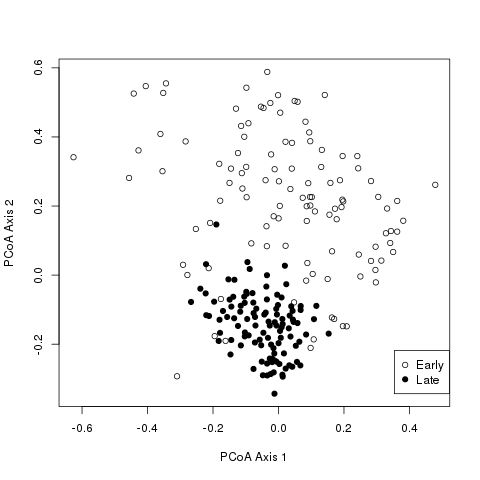
\includegraphics{../results/figures/nmds_figure.png}
\end{figure}

\newpage

\subsection{References}\label{references}

1. \textbf{Schloss PD}, \textbf{Schubert AM}, \textbf{Zackular JP},
\textbf{Iverson KD}, \textbf{Young VB}, \textbf{Petrosino JF}. 2012.
Stabilization of the murine gut microbiome following weaning. Gut
Microbes \textbf{3}:383--393.
doi:\href{http://dx.doi.org/10.4161/gmic.21008}{10.4161/gmic.21008}.

2. \textbf{Yue JC}, \textbf{Clayton MK}, \textbf{Lin F-C}. 2001. A
nonparametric estimator of species overlap. Biometrics
\textbf{57}:743--749.
doi:\href{http://dx.doi.org/10.1111/j.0006-341x.2001.00743.x}{10.1111/j.0006-341x.2001.00743.x}.

\end{document}
